%% 
%% Copyright 2019-2020 Elsevier Ltd
%% 
%% This file is part of the 'CAS Bundle'.
%% --------------------------------------
%% 
%% It may be distributed under the conditions of the LaTeX Project Public
%% License, either version 1.2 of this license or (at your option) any
%% later version.  The latest version of this license is in
%%    http://www.latex-project.org/lppl.txt
%% and version 1.2 or later is part of all distributions of LaTeX
%% version 1999/12/01 or later.
%% 
%% The list of all files belonging to the 'CAS Bundle' is
%% given in the file `manifest.txt'.
%% 
%% Template article for cas-sc documentclass for 
%% double column output.

%\documentclass[a4paper,fleqn,longmktitle]{cas-sc}
\documentclass[a4paper,fleqn]{cas-sc}

% \usepackage[numbers]{natbib}
%\usepackage[authoryear]{natbib}
\usepackage[authoryear,longnamesfirst]{natbib}
\usepackage{algorithm}
\usepackage{multicol}
\usepackage{algpseudocode}
 \usepackage{subcaption}
%%%Author definitions
\def\tsc#1{\csdef{#1}{\textsc{\lowercase{#1}}\xspace}}
\tsc{WGM}
\tsc{QE}
\tsc{EP}
\tsc{PMS}
\tsc{BEC}
\tsc{DE}
%%%

% Uncomment and use as if needed
%\newtheorem{theorem}{Theorem}
%\newtheorem{lemma}[theorem]{Lemma}
%\newdefinition{rmk}{Remark}
%\newproof{pf}{Proof}
%\newproof{pot}{Proof of Theorem \ref{thm}}

\begin{document}
\let\WriteBookmarks\relax
\def\floatpagepagefraction{1}
\def\textpagefraction{.001}

% Main title of the paper
\title [mode = title]{Local planning via Multi-Agent DMPC techniques applied to platoons of autonomous vehicles.}                    

% First author
%
% Options: Use if required
% eg: \author[1,3]{Author Name}[type=editor,
%       style=chinese,
%       auid=000,
%       bioid=1,
%       prefix=Sir,
%       orcid=0000-0000-0000-0000,
%       facebook=<facebook id>,
%       twitter=<twitter id>,
%       linkedin=<linkedin id>,
%       gplus=<gplus id>]
\author[1,2]{Marc Facerias}[                   orcid=0000-0001-7511-2910]

% Email id of the first author
\ead{marc.faceriaspelegri@manchester.ac.uk}

% Address/affiliation
\affiliation[1]{organization={University of Manchester},
    city={Manchester},
    % citysep={}, % Uncomment if no comma needed between city and postcode
    % state={},
    country={United Kingdom}}
    
% Third author
\author[2]{Vicenç Puig}
\ead{vicenc.puig@upc.edu}

% Address/affiliation
\affiliation[2]{organization={Universitat Politecnica de Catalunya},
    % addressline={}, 
    city={Barcelona},
    % citysep={}, % Uncomment if no comma needed between city and postcode
    country={Spain}}

% Second author
\author[1]{Alexandru Stancu}
\ead{alexandru.stancu@manchester.ac.uk}
% Here goes the abstract
\begin{abstract}
This work explores the development of a local collaborative planning algorithm for autonomous agents. In particular two novel approaches are proposed, a decentralised quadratic planner and its distributed counterpart based on the Optimality Condition Decomposition algorithm. Both strategies have proved to be suitable in different domains and in this paper their applicability to the autonomous driving domain is tested by applying them in a Highway-like scenario.  
\end{abstract}

% Use if graphical abstract is present
% \begin{graphicalabstract}
% \includegraphics{figs/grabs.pdf}
% \end{graphicalabstract}

% Research highlights
% \begin{highlights}
% \item Research highlights item 1
% \item Research highlights item 2
% \item Research highlights item 3
% \end{highlights}

% Keywords
% Each keyword is seperated by \sep
\begin{keywords}
LPV-DMPC \sep
Local Planning \sep 
Distributed Optimisation \sep 
\end{keywords}


\maketitle

\section{Introduction}
\label{seq:Intro}
In the last few years, the automotive sector has been advancing more and more towards the automatising of transport systems, with autonomous cars being few years away from a general public adoption. In this context of hyperconected autonomous devices it is expected to see a paradigm shift, from the roads being streams of independent agents competing with each other to reach their goal to a flow of interconnected entities that seek to accomplish their objectives through peer to peer collaboration. Due to the advances of V2V, vehicle to vehicle, and V2I, vehicle to infrastructure, communication protocols allowing fast data transition between agents and with external elements it has become a matter of interest to propose collaborative algorithms for autonomous driving.\\ 

Autonomous driving, and thus collaborative driving, can not be considered an unique problem, as there exists a wide range of scenarios that involve different behaviours. Consequently, current research is focused on solving individual sub-problems, such as intersection management \cite{Pei2021}, assistive driving \cite{medero2021control}, platooning \cite{Vlachos2022} or lane changes \cite{LaneChangeXie2021} etc. In this work, we fall within the platooning category, even though our approach follows a different philosophy than the one present in most research lines.\\ 

Platooning is considered to be the problem of managing a group of agents that aim to keep a certain formation, both in terms of position and velocity, while traversing a common environment. It can be seen that this definition matches the behaviour that naturally appears in highways, a set of vehicles keeping a security distance between each other and driving close to the maximum allowed velocity. However, when done in an informed manner, an structured navigation proved to lower fuel
consumption, reduce $CO_2$ emissions and improve traffic fluency \cite{FuelMinimisation}. Typically, this fleets rely on having either a predefined desired formation to follow, as shown in \cite{FormationControlDistri}, or there is a leader-follower relationship between agents, where a leader dictates the path and the followers maintain a certain distance or velocity with respect to it \cite{Liu2017}.  However, we aim to work with an structure more natural to the human interaction, where agents communicate between each other to arrange themselves in a formation that benefits not only their individual goals but the collective behaviour of the group. \\ 

In general, what is going to define the design of a multi-agent network is the communication topology that governs the system, as the level of information available to each agent determines the degree of dependency between elements in the network. In this context we can find three different scenarios.
\begin{itemize}
    \item Centralised systems: All systems are completely dependent from the other agents in the network, and the decision making is handled by a central unit that defines the behaviour of the rest to optimise some global metric. 
    \item Distributed systems: Each agent computes an individual problem which is refined through an iterative algorithm to reassemble a centralised optimisation, taking into account the information of their peers to deal with any coupling present in the system. 
    \item Decentralised systems: Each agent accounts for their individual goal by either relaxing or ignoring the coupling behaviour. In this case, individual agents account for their peers mostly for safety features such as collision avoidance either by using onboard sensors or through basic communication.  
\end{itemize}

Centralised approaches have fallen out of fashion within the robotics community, as with the improvement of communication and computing capabilities of small robots it is more flexible and reliable to make the system modular rather than to trust a single individual. However, there are some recent examples in the field where this architecture is still used. Some of them can be found in \cite{Wang2016}, where a central unit decides whether or not an overtaking manoeuvre should be performed. In another line of work, \cite{Queralta2020} relies on a centralised goal assignment algorithm and locally each individual is equipped with an obstacle avoidance module and low level controller to reach the desired position. \\ 

Distributed solutions remain popular within the community, as with the current communication technologies they provide a good trade-off between global performance and latency of the algorithm. In \cite{DistriADMM} the alternating direction method of multipliers (ADMM) algorithm is applied, being the main innovation with respect to other lines of work the usage of a spline based characterisation of the environment. In similar lines of work, \cite{Vlachos2022} presents a platooning ADMM algorithm with a leader-follower structure and evaluates its performance in Carla, a high-fidelity simulator for autonomous driving. A distributed collision avoidance approach is presented in \cite{8550245}, where simple agents modelled through a double integrator are coordinated using ADMM and a linear approximation of the collision avoidance constraints that allow solving the problem in a simpler manner. Similarly, \cite{van2016online} presented an ADMM coordination strategy that relies on separating lines for obstacle avoidance and spline-based trajectory characterisation, showing how the distributed algorithm improved the results of its centralised counterpart. Moreover, distributed coordination strategies allow system reconfiguration in an ad-hoc manner, preventing local failures to compromise the whole system. An example of this behaviour can be found in \cite{adHoc2021}, where a novel online platoon reconfiguration technique is presented and compared to the current European standards, with an special focus on the physical limitations that need to be overcome to implement this family of algorithms. In another line of work, \cite{8648233} proposes an ADMM optimal consensus controller applied to systems of particles. Interestingly, other approaches do not rely on optimising a common performance metric to force a collaborative nature. For instance, in \cite{8648233} a game theoretic approach based on Gauss-Seidel iterative method is proposed, allowing agents to decide whether to compete or collaborate, achieving a more human-like behaviour while improving their  performance compared with a classic MPC.\\ 

Decentralised algorithms switch the paradigm of the two scenarios presented and decouple each subsystem by ignoring their interactions. In other words, we effectively assume that global performance is subject to maximising the performance of each individual in an isolate manner, leading to a more competitive behaviour which opposes the collaborative nature of other architectures. For instance, in \cite{Hult2019} presents a decentralised solution for the navigation in road intersections where each agent acts individually and a second coordination layer gives priority to each of them in a centralised manner to minimise the cost related to its intersection. In another line of work, \cite{Lee2020} presents a platooning algorithm with an special focus on the physical implementation of the network with a real fleet of trucks. Similarly, \cite{Regragui2023} presents an urban navigation network where agents communicate with devices installed in the streets that assign plans seeking to optimise the routes in a collaborative manner. Note that the decentralised approaches do not require a common global cost function, instead the system design is such that a distributed optimisation is not required, typically by adding some kind of control device handling the cooperation, that somehow resembles a centralised implementation. This strategies are adopted due to the fact that, as presented in \cite{guillaume2008fast}, ignoring interaction between agents  in highly coupled systems may lead to degraded solutions. \\

Regarding the interaction between agents, most algorithms rely on the geometric relationship between them. As it can be seen in \cite{Frenet2022} where a collection of metrics is presented and evaluated to prevent collision between agents and the environment. However, other approaches treat collision avoidance through the expected interaction between subsystems. We found of particular interest the use of potential field functions \cite{Rasekhipour2017}, which allow the system to evolve in a less constrained manner by assigning repulsive forces to obstacles and attractive forces to goals. Similarly in \cite{Song2013} the elastic band theory is used to deform the expected path to adapt it to the environment conditions, for instance doing a line change to overtake an slow vehicle.\\

So far, most of the work presented rely on some sort of optimisation technique embedding different performance metrics and levels of interaction between agents. However, it is worth to mention less orthodox techniques that inspired by other trends in the robotics field present alternative formulations. We found of particular interest the work of \cite{Bae2019}, where the planning policy is learned by trying to improve the performance of an $A^*$ algorithm. In another line of work \cite{Wang2022} uses probabilistic based approaches to generate a set of possible trajectories from a base curve and then the preferred candidate is selected ensuring a collision free trajectory. Note that probabilistic approaches tend to involve some sort of optimisation problem that selects the final trajectory not only taking into account collisions but other performance metrics, being an example \cite{Heintzman2021}.\\

In this paper, we aim to propose a novel distributed approach based on the Optimal Condition Decomposition (OCD) algorithm and a relaxed version that solves the problem in a decentralised manner using Linear Parameter Varying (LPV) models. To the best of our knowledge the proposed approaches have not yet been explored in the context of a cooperative autonomous driving. Furthermore, while most of the literature require some sort of central coordination unit to either relax or coordinate the optimisation, we aim to solve in a fully distributed manner. The main contributions of this research are the following: 

\begin{itemize}
    \item Propose a distributed planning algorithm using Optimal Condition Decomposition.
    \item Propose a decentralised LPV-MPC cooperative planning algorithm. 
    \item Analyse the performance of both algorithms in a test track resembling a highway. 
\end{itemize}

Finally, the paper is structured as follows. In Section \ref{sec:Preambles} the techniques used as a baseline for the development of the rest of the paper are introduced, along with the notation that is going to be followed. In Section \ref{Sec:MA optimal plans} the context of multi-agent planning problems is presented and the proposed algorithms are defined in a general manner. In Section \ref{seq:CaseStudy} the work is particularised into the highway platooning problem and the testing environment is presented. Section \ref{seq:exp} contains the results of applying the proposed algorithms along with an extensive performance review. Finally, In Section \ref{sec:Conclusions} we discuss the results of the paper and the future work. 

% ------------------------------------------------------------------------------
% ------------------------------------------------------------------------------
\section{Preambles}
\label{sec:Preambles}
\subsection{Notation}
\begin{itemize}
    \item $f(\cdot)$: Arbitrary function
    \item $x^k_n$: $n^{th}$ agent instance of an arbitrary variable $x$ evaluated in the time instant $k$ 
    \item $\vartheta^{k,n,j}$: Parameter vector defining a plane in a $\mathbb{R}^2$ space, linked to time instant $k$ and agents $n,j$ defined as $\vartheta^{k,n,j} = [\vartheta_{1}^{k,n,j},\vartheta_{2}^{k,n,j},\vartheta_{3}^{k,n,j}]$
    \item $\vartheta_{1,2}^{k,n,j}$: First and second coefficients of the plane $\vartheta^{k,n,j}$
    \item $x$: states involved in an optimisation problem. 
    \item $u$: control actions involved in an optimisation problem
    \item $\underline{x}, \overline{x}$ : Lower and upper bounds of an arbitrary variable $x$. 
    \item $\lambda^g_{k,n}$: Lagrange multiplier associated to the $g$ constraint of agent $n$ at time instant $k$. 
    \item $I_n$: $nxn$ identity matrix. 
    \item $H$: Prediction horizon of a control problem. 
    \item $\hat x$: Current approximation of an arbitrary variable $x$. In the context of an iterative algorithm used to represent current value of a variable being updated.
    \item $p^{k}_j$: Position vector of agent $j$ at time instant $k$, defined as the $x$ and $y$ coordinated of its center of gravity with respect to a global frame. Note that is defined as $p^{k}_j = [x,y,1]$, being $x$ and $y$ the coordinates of the agent in a $\mathbb{R}^2$ space. 
    \item $\lVert \cdot \rVert_n$ : Norm of type $n$.
\end{itemize}

\subsection{Model Predictive Control}
The baseline tool that we are going to use in this paper is known as Model Predictive Control (MPC), which is a finite horizon model-based optimisation technique widely used in the control community. However, due to its usage of an embedded system model it is also common to generate not only control actions, but trajectories to be followed by the agents. The main motivation of using this technique is that it naturally embeds the complexity of our system model, along with any performance constraints that the designer may add into the system. In comparison, classical planning techniques tend to focus more on the spatial setting to be traversed, while the specific dynamics of the agents tend to be either simplified or ignored, using a lower layer of control the role of generating the specific signals that will drive the agent as close as possible to the desired behaviour, being an example \cite{AlonsoPuntualModel}. In this context, the architecture of an MPC allows us to treat easily the possible collisions and road limitations while using a detailed vehicle model, thus the plans generated are realistic and provide an additional layer of security towards the user.\\ 

In general, any optimisation problem can be presented as follows.  
\begin{equation}
\begin{aligned}
\min\limits_{x}  &\quad f(x) &\\ 
s.t.             &\quad g_i(x)=0, & i = 1,...,m\\
&\quad h_j(x)\leq0, &j = 1,...,n
\end{aligned}
\end{equation}

where $f(x)$ refers to a cost function to be minimised by the selection of a suitable $x$ while satisfying an arbitrary number of equality and inequality constraints, represented by $g_i(x)$ and $h_j(x)$ respectively.\\

MPC is a particular formulation of this problem and its general structure is introduced in Eq. \eqref{MPC}. Note that this formulation along with some of its many variations can be found in \cite{Bai2019}.
\begin{equation}
\label{MPC}
\begin{aligned}
\min\limits_{x,\Delta u}  &\quad J=\sum_{i=1}^{N} (r_i-x_i)w_{x_i}(r_i-x_i) +  \sum_{i=1}^{N} \Delta u_i w_{u_i}\Delta u_i&\\ 
s.t.             &\quad x_{i+1}=f(x_i)\\ 
&\quad \underline{u} \leq u_{i-1} + \Delta u_i \leq \overline{u}
\end{aligned}
\end{equation}
An MPC controller is based on computing a series of optimal control actions within a horizon $N$ that both regularise the variation of $u$ and minimise the difference between the current state $x_i$ and the desired state $r_i$ where $i = 1,...,N$, note that there are two weighting factors $w_{x_i}$ and $w_{u_i}$ that allow to bias the optimisation problem towards any of the terms involved. By adapting this structure can compute a control action $u_i$ while considering the optimal variations of states that ensure our system follows the reference trajectory. In order to do so, we introduce an equality constraint $f(x)$ containing the system model that allows us to predict how is our system going to evolve. Additionally, inequality constrains can be used to bound the admissible values of the control action or any other system characteristic required by our application.  \\

It needs to be taken into account that any optimisation problem comes with certain limitations by nature, as it is not always possible to find an unique global minima. In particular, guaranteeing to find a global optimal is subject to the convexity of the cost function and the linear nature of its constraints. If any of this conditions is not satisfied e.g., the cost function is non-convex or either $f(x)$ or $g(x)$ are not linear, the solution may either be a local minima or lead to computational times prohibitive for an online implementation. Typically, the convexity of the cost function is ensured by defining it in a suitable form while issues with the non-linearity of the systems are addressed with some sort of linearisation technique, such as Taylor series. It is worth to note that in many cases non-linear optimisation problems are solved regardless the limitations presented, being an example \cite{gao2010predictive}. Other techniques such as Real Time Iteration avoid the complexity of having to use a purely non-linear solver by relying on solving a single Newton iteration of consecutive optimisation problems, as presented in \cite{RTI}, where the proposed algorithm solves a non-linear MPC with computational times close to its linear counterpart. However, their performance tends to be quite sensitive to the nature of the non-lineraties present in the system and the initial conditions chosen for the optimisation.\\

% ------------------------------------------------------------------------------
% ------------------------------------------------------------------------------

\subsection{Lagrangian relaxation methods }
Lagrangian relaxation methods are techniques applied to optimisation problems that aim to solve a simplified, relaxed, version of the problem through the application of the Lagrange multipliers. In order to illustrate this concept, we will introduce an arbitrary optimisation problem in Eq. \eqref{eq:LR example}. 

\begin{equation}
\label{eq:LR example}
\begin{aligned}
    & \underset{x}{\text{min}}f(x) \\
    & \text{s.t.}\\
    &&& h(x) \leq 0 \\
\end{aligned}
\end{equation}

Considering we want to relax Eq. \eqref{eq:LR example} the constraint $h(x)$ can by added to the cost function through a term $\lambda$, known as a Lagrange multiplier, leading to $\underset{x}{\text{min}}f(x) + \lambda h(x)$.\\ 

It can be observed that the problem is enforced to minimise the term $\lambda h(x)$, which for an appropriate positive value of $\lambda$ is equivalent to treating $h(x)$ as a constraint. This same principle is exploited by several decomposition techniques, which take advantage of embedding certain coupling constraints as part of the cost function to solve the complete problem in a distributed manner. Even though there is a vast literature regarding the solution of this distributed problems, they can be classified as either Lagrangian decomposition or decentralised solution of the KKT conditions for local optimality \cite{kargarian2016toward}. Two of the most popular techniques are the ADMM and the optimality conditions decomposition
(OCD), and pertain to the first and second approaches, respectively. \\ 

It can be seen that among the literature presented in Section \ref{seq:Intro} ADMM is the most extended technique and, even though OCD is similar in essence, the latter presents some advantages that allow a system topology more convenient for the problem treated in this paper. As presented in \cite{Segovia2021}, the main advantage of OCD over ADMM is that the latter does require a central coordination unit to perform the dual variable update, while OCD only requires communication with peers that present coupling with each other. This key difference in the system structure not only avoids relying on a specific agent but opens the door to the implementation of security features and dynamic agent reallocation in a simpler manner. \\


As mentioned before, OCD is a technique based on the Lagrangian decomposition method, proposed in  \cite{conejo2006decomposition}, that aims to divide a complex problem into simpler sub-problems by separating the coupled constraints. In this context, consider an optimisation problem with two groups of variables $x = [x_1, x_2]$, as shown in Eq. \eqref{eq:OCD example}. 
\begin{equation}
\label{eq:OCD example}
\begin{aligned}
    & \underset{x_1,x_2}{\text{min}}f(x_1,x_2) \\
    & \text{s.t.}\\
    &&& g_1(x_1) \\
    &&& g_2(x_2) \\
    &&& h_1(x_1,x_2)\\
    &&& h_1(x_1,x_2)\\
\end{aligned}
\end{equation}
In this example we consider $g_i$ separable constraints, which involve only one subset of states, while $h_i$ are constraints that do not allow a direct decomposition. This can be solved by fixing a certain subset of variables, leading to two problems of the shape presented in Eq. \eqref{eq:OCD Dexample}. For clarity purposes we will not write the second half of the distributed problem, as it can be obtained by switching indexes $1$ and $2$. 
\begin{equation}
\label{eq:OCD Dexample}
\begin{aligned}
    & \underset{x_1}{\text{min}}f(x_1,\hat{x}_2)) + {\lambda_2} h_2(x_1,\hat{x}_2)\\
    & \text{s.t.}\\
    &&& g_1(x_1) \\
    &&& h_1(x_1,\hat{x}_2)\\
\end{aligned}
\end{equation}
Then we are going to iterate through the update algorithm in Alg. \ref{alg:NL planning algorithm} to compute an approximation of the optimal solution to the problem. It is worth to note that any update policy of $\alpha$ could be applied to improve the convergence rate of $\lambda$, but for simplicity purposes a constant positive update rate has been used in this formulation. 

\begin{algorithm}[h]
\caption{Distributed planning algorithm for an agent $n$ with neighbour $i$}
\label{alg:NL planning algorithm}
\While{not convergence}
   \State Collect current $x_i$ and set $\hat{x}_i = x_i$
   \State Update ${\lambda_n} = {\lambda_n} + \alpha h(x^k_i,x^k_n)$
    \State Compute a step of $i_{th}$ optimisation problem
    \State Forward $x_n$ thorough the system
\EndWhile
\end{algorithm}


\subsection{Linear Parameter Varying Models}
\label{sec:LPV_Mod}

Linear Parameter Varying systems are defined as finite-dimensional linear time-varying models whose state space matrices are fixed functions of some vector of varying and measurable parameters, as defined by \cite{sename2013robust}. We aim to rearrange an arbitrary nonlinear model of the form $x_{k+1} = f(x_k,u_k)$ so that it has the shape $x_{k+1} = A(\zeta)x_k + B(\zeta)u_k$. It can be seen that the latter form resembles a linear model with respect to $x$ and $u$. Note that this is will be only strictly linear as long as $A(\zeta)$ and $B(\zeta)$ are independent from $x$ and $u$, which in general can not be assumed for non-linear systems. In order to overcome this limitation $\zeta$ is defined as a set of varying parameters that can be measured and fixed for a given time instant $k$, leading to a linear model.\\ 

An example of this technique can be found in the well known bicycle model, represented by a nonlinear set of differential equations in Eq. \eqref{eq:bycicle}.\\ 
    \begin{equation}
        \begin{aligned}
            \label{eq:bycicle}
            &&& \dot{p_x} = v * cos(\theta) \\
            &&& \dot{p_y} = v * sin(\theta) \\
        \end{aligned}
    \end{equation}
It is obvious to see that the model presented is non-linear with respect to $u$, so following an LPV philosophy we will rearrange it in a pseudo-linear form in Eq. \eqref{eq:LPV} by redefining $x$ and $u$ as $x = [p_x,p_y]$, representing the Cartesian coordinates of the robot, and $u = [v,\theta]$, representing its linear velocity and heading.\\ 
\begin{equation}
\label{eq:LPV}
    \dot{x} = \left[\begin{array}{cc}
                \frac{cos(\theta)}{\theta} & 0 \\
                0 & \frac{sin(\theta)}{\theta} \\
            \end{array}\right] u 
\end{equation}

Note that as mentioned before, this model can be treated as linear as long as the value of $\theta$ is fixed. It is worth to note that due to the presence of an scheduling vector $\zeta$ polytopic interpolation techniques are required to instantiate the model at ${\zeta_k}$. However, in this particular case due to the nature of MPC techniques an estimated ${\hat{\zeta}}$ can by generated, allowing the application of linear solvers to non-linear models without the need of a formal linearisation. More extensive theory about the polytopic use of LPV models and their applications can be found in previous works done within the research group, such as \cite{facerias2022zonotopic}. The performance of the resulting model may vary depending on the nature of the non-liniarities present in the original model, being in some cases impossible to generate an LPV model. However it proved to be suitable for this application, being its results close to the nonlinear counterpart \cite{alcala2019lpv}.

\subsection{Obstacle avoidance in collaborative autonomous systems}
    \label{sec:obs_avoidance}

    As it was seen in previous sections of this paper, the degree of inter-vehicle communication has a great impact on the design techniques involved in the optimisation algorithms. This is specially relevant when considering obstacle avoidance, as the better information available from a neighbouring agent the better it will be represented in the subsequent optimisation problem. In this work two different techniques will be explored, separating hyperplanes and the Euclidean distance between agents.\\
    
    The separating hyperplanes technique is based on fitting an hyperplane between two vehicles. In order to illustrate this, we will separate a pair of vehicles $i$, $j$ by an hyperplane, as it can be seen in Fig. \ref{fig:figPlane}. In this pair $i$ is considered the ego vehicle and $j$ is considered the neighbour. The existence of such hyperplane implies that the points representing the center of gravity are not superposed.  This is imposed by finding the parameter set $\vartheta$, which defines a plane in $\mathbb{R}^2$, that satisfies Eq. \eqref{eq:plane} for a pair of points $x,y$. Note that this formulation can be extended to consider the agents not punctual, but bounded by any polygonal shape we desire by taking $x = [x_1,x_2, ... x_N]$ and $y = [y_1,y_2, ... y_N]$, being $x$ and $y$ sets containing the vertices of an $N$ dimensional polygon. However, this adds an additional computational burden to the system as the number of constraints increases, thus it was decided to use a safety band around the separating hyperplane wide enough to prevent collision between vehicles through the term $D_{sf}$. Note that a normalisation constraint is added to prevent degenerate solutions. Furthermore, exchanging $x$ and $y$ in Eq. \eqref{eq:plane} will result in an equal plane of inverted sign, which is equivalent in terms of the spacial separation of the agents.\\ 
    \begin{equation}
        \begin{aligned}
            \label{eq:plane}
            &&& \vartheta x \leq -\frac{D_{sf}}{2} \\
            &&& \vartheta y \geq \frac{D_{sf}}{2} \\
            &&& \lVert \vartheta_{1,2} \rVert_2 = 1 
    \end{aligned}
    \end{equation}
    On the other hand, Euclidean distance is a well known metric that by bounding the maximum allowed distance between agents creates a circular exclusive region around each robot, which is represented both graphically and numerically by Eq. \eqref{eq:euclidean} and Fig. \ref{fig:figEuclidean}, respectively. It is trivial to see that collision avoidance is achieved as long as the region encloses the vehicle. 
    
    \begin{equation}
        \begin{aligned}
            \label{eq:euclidean}
            &&& \lVert x - y \rVert_2 \geq 2*E_{sf} \\
        \end{aligned}
    \end{equation}

\begin{figure}
    \centering
        \begin{subfigure}{0.5\textwidth}
          \centering
          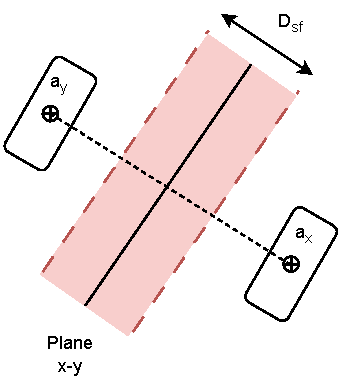
\includegraphics[width=.7\textwidth]{figs/Planes.drawio.pdf}
          \caption{Separating Hyperplanes}
          \label{fig:figPlane}
        \end{subfigure}%
        \begin{subfigure}{.5\textwidth}
          \centering
          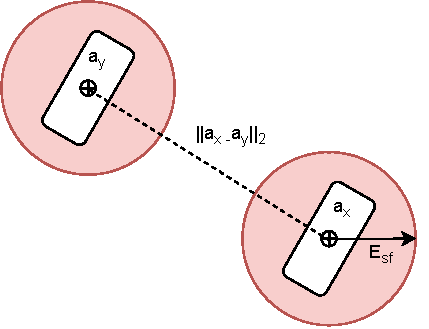
\includegraphics[width=.7\textwidth]{figs/Euclidean.drawio.pdf}
          \caption{Euclidean distance}
          \label{fig:figEuclidean}
        \end{subfigure}
    \caption{Separation of two agents $a_x$ and $a_y$, being highlighted in red the regions considered to be excluded due to the risk of collision.}
    \label{fig:DistanceMetrics}
\end{figure}
    
    They main difference between this two techniques is on how over-constrained the solution space is with respect to the agents. As it can be seen, a circular region typically will be over-approximating the rectangular shape of a vehicle, which could lead on performances losses. However it proves to be easier to implement in terms of both the number of constraints and variables involved. On the other hand, separating hyperplanes allow a better description of the surrounding region at the cost of having a more complex numerical problem. As an additional remark, separating hyperplanes are linear with respect to the variables $x$ and $y$ while using $l^2$ norm involves having to compute an optimisation problem with nonlinear constraints. This characteristic opens the door of computing an online approximation of $\vartheta$ thus relaxing the optimisation problem, as it will be seen in further sections of this paper. It is worth to note that other geometrical shapes may improve the coverage issues present in the Euclidean distance, as it can be seen in \cite{Frenet2022} where both ellipses and overlapped circles were used to provide an accurate representation of the agent surface. 
%------------------------------------------------------------------------------
\section{Multi-Agent Optimal Planning}
\label{Sec:MA optimal plans}
\subsection{Problem statement}
The collaborative planning problem can be defined as the search of suitable paths for a group of agents that allow navigating an environment while satisfying a set of constraints. This constraints will vary depending on the nature of the system, being in this specific scenario the physical limits of the agents and the safety margins between them. The main complication associated with this type of problems is that in order to find a suitable path for each vehicle we need to embed all the agents of the system in a single optimisation problem, which can lead to idle times too big for any real time application. Furthermore, solving a single optimisation problem implies that the system needs a central computing unit and a communication network powerful enough to ensure the propagation of the solutions and retrieving of all the individual agent data.\\ 

The inherent fragility and inefficiency of the centralised approach motivated the reformulation of the problem in a distributed manner. Even though there is still a performance bottleneck related with the latency of the network, we can solve $N$ optimisation sub-problems locally while achieving an optimality degree close to the centralised case through the propagation of local solutions and solving the sub-problems iteratively until convergence. This approaches tend to present algorithm with a high computational load, thus an alternative can be found in decentralised optimization approaches, which are a relaxed version of the original problem that either ignore the coupling between subsystems or rely on an approximation of their local variables, leading to a set of $N$ independent problems.\\ 

Solving the problem in a distributed fashion has a bigger computational cost involved, both in terms of communication burden and the optimisation time, but it provides a solution closer to its centralised counterpart considering a stopping criteria properly defined. On the other hand, decentralised approaches prioritise the computational time over the global performance of the system, which may lead to a poor global behaviour.\\ 

In a general manner, the steps followed to synthesise any of the proposed controllers are the following: 

\begin{enumerate}
  \item Define the global function of the network and identify the subsystems, which in this case is trivial due to the nature of the problem, and define the information exchange.
  \item Define the coordination strategy between the subsystems, which will depend on the architecture of the algorithm.
  \item Synthesise the local implementations of the multi-agent algorithm. 
\end{enumerate}\\ 

In further sections of this paper both decentralised and distributed control strategies will be synthesised and applied to the autonomous driving domain to study their performance. 

\subsection {Non Linear DMPC formulation }
\label{NL MPC}
In other to propose a distributed control problem we will start by analysing its centralised counterpart, which in this case is equivalent to consider all the vehicles in the road and their interactions as a single system. 

\begin{equation}
\label{eq:opt problem}
\begin{aligned}
    & \underset{\Delta u^k_n}{\text{min}}  &&\mathrm{J}=\sum_{k=0}^{H} \sum_{n=0}^{N}( J^k_n(x^k_n)) \\
    % .....................
    & \text{s.t. $\forall k \in [0,H], \forall n \in [1,N]$}\\
    &&& x^{k+1}_n = f(x^{k}_n,u^{k}_n)\\
    &&& u^k_n = u^{k-1}_{n} + \Delta u^k_n \\ 
    &&& u^k_n \in [\underline{u^k_n}, \overline{u^k_n} ] \\
    &&& e_{y_{n}}^{k} \in [\underline{e_{y_{n}}^{k}}, \overline{e_{y_{n}}^{k}} ] \\
    % .....................
    & \text{s.t. $ \forall k \in [0,H], \forall n \in [1,N] ,\forall j \in [1,N]\ j \neq n $}\\
    &&& g(\vartheta^{k,n,j},p^{k}_n) \equiv \vartheta^{k,n,j} p^{k}_n <= \frac{-D_{sf}}{2} \\
    &&& h(\vartheta^{k,n,j},p^{k}_j) \equiv \vartheta^{k,n,j} p^{k}_j >= \frac{D_{sf}}{2} \\
    &&& \lVert \vartheta^{k,n,j}_{1,2} \rVert_2 = 1 \\
\end{aligned}
\end{equation}

\noindent where $J^k_n(x^k_n)$ has the following quadratic shape:
\begin{equation}
    J^k_n(x^k_n) = xQx + \Delta u Q_u \Delta u + q_xx + q_uu + q_{\sigma}\sigma
\end{equation}

Being $x$ the vehicle states, $u$ the control variables, $e_{y_{i}}^{k}$ the lateral error and $\sigma$ a set of slack variables. $Q$, $q_x$, $q_u$ and $q_{\sigma}$ are weighting factors applied to each variable. Finally, both $g$ and $h$ are the constraints associated to the separating hyperplanes\\ 

Applying OCD to Eq.\eqref{eq:opt problem} leads to $N$ subsystems which shape vary depending on their communication topology. In order to exemplify their structure we are going to present a simplified case with two agents $a_1$ and $a_2$. Keep in mind that for the constraint representation the heuristics presented in Section \ref{sec:obs_avoidance} have been taken into account. Eq. \eqref{eq:ego_agent} refers to $a_1$ while in Eq.\eqref{eq:slave_agent} refers to $a_2$. 

\begin{equation}
\label{eq:ego_agent}
\begin{aligned}
    & \underset{u_k}{\text{min}} && \mathrm{J}=\sum_{k=0}^{H} ( J^k_1(x^k_1) + J^k_2(\hat{x}^k_2)) + \lambda^h_{1,2}h(\vartheta^{k,n},\hat{p}^k_2)\\
    & \text{s.t. $\forall k \in [0,H]$}\\
    &&& x^{k+1}_1 = f(x^{k}_1,u^{k}_1)\\
    &&& u^k_1 = u^{k-1}_{1} + \Delta u_1 \\ 
    &&& u^k_1 \in [\underline{u^k_1}, \overline{u^k_1} ] \\
    &&& e_{y_{1}}^{k} \in [\underline{e_{y_{1}}^{k}}, \overline{e_{y_{1}}^{k}} ] \\
    % .........
    &&&  g(\vartheta^{k,1,2},p^{k}_1)  \\
    &&& \lVert \vartheta^{k,1,2}_{1,2} \rVert_2 = 1 \\
\end{aligned}
\end{equation}

\begin{equation}
\label{eq:slave_agent}
\begin{aligned}
    & \underset{\Delta u^k_n}{\text{min}} && \mathrm{J}=\sum_{k=0}^{H} ( J^k_2(x^k_2) + J^k_1(\hat{x}^k_1)) \\
    % ........
    & \text{s.t. $\forall k \in [0,H]$}\\
    &&& x^{k+1}_2 = f(x^{k}_2,u^{k}_2)\\
    &&& u^k_2 = u^{k-1}_{2} + \Delta u^k_2 \\ 
    &&& u^k_2 \in [\underline{u^k_2}, \overline{u^k_2} ] \\
    &&& e_{y_{2}}^{k} \in [\underline{e_{y_{2}}^{k}}, \overline{e_{y_{2}}^{k}} ] \\
    &&& h(\hat{\vartheta}^{k,1,2},p^{k}_2) \\
\end{aligned}
\end{equation}

As it can be seen, applying this formulation as presented in Eq. \eqref{eq:opt problem} leads to duplicated constraints due to having equivalent planes. Specifically, when dealing with an arbitrary pair $i$ and $j$ two equivalent planes are generated, as $\vartheta^{k,i,j} \equiv \vartheta^{k,j,i}$. In order to prevent duplicating constraints we applied the following heuristics:     
    
    \begin{itemize}
        \item if $i<j$ we will consider $i$ as the ego vehicle and add the constraint $g(\vartheta^{k,n,j},p^{k}_n)$ to its optimisation problem. With this distribution we associated the plane states to the vehicle $i$ and the term $\lambda^h_{1,2}h(\vartheta^{k,n},\hat{p}^k_2)$ is added to consider the neighbouring agent. 
        \item if $i>j$ we will consider $j$ as the neighbour and its obstacle avoidance constraint related to $i$ is treated through $h(\vartheta^{k,n,j},p^{k}_j)$. 
    \end{itemize}

Its trivial to see that applying this heuristics to a pair $i,j$ results in only one plane being generated, either $\vartheta^{k,i,j}$ or $\vartheta^{k,j,i}$, depending on the numeric id associated to each agent.\\
    
Additionally, slack variables $\sigma_u$, $\sigma_{e_y}$, $\sigma_g$, $\sigma_h$ were added to the system and introduced in the cost function with appropriate weighting factors. This variables allow the constraints associated to them to be violated, however this dramatically increases the cost function value. Thus, it will only happen in situation that otherwise would lead to system deadlocks, e.g a bottleneck where the only way to advance is by being closer than $D_{sf}$. \\ 

As mentioned before, adding the separating hyperplanes as part of the optimisation problem leads to a better representation of free space, however it comes with an increased computational burden over the system. For this reason an alternative formulation to Eq. \eqref{eq:opt problem} was proposed by substituting the terms related to the plane computation by their Euclidean counterpart, while keeping the same heuristics presented in this section. 

\subsection{LPV - DMPC}
\label{sec:LPV - DMPC}
It can be seen that the complexity of solving Eqs \eqref{eq:ego_agent} \eqref{eq:slave_agent} is considerable, as it involves solving several iterations of a non-linear optimisation problem. This motivated the relaxation of the OCD formulation into a decentralised quadratic problem, which is going to be introduced in this section. Firstly, due to the highly nonlinear nature of Eq. \eqref{NL MPC}, a LPV model, with the structure of Eq. \eqref{eq:LPV model structure}, was introduced into Eq. \eqref{eq:opt problem}. 

\begin{equation}
    \label{eq:LPV model structure}
    x^{k+1}_i = x^{k}_i + ( A_i(\zeta^{k}_i) x^{k}_i + B_i(\zeta^{k}_i) u^{k}_i ) T_s
\end{equation}

It is expected that this relaxation improves the inherently slow computational time of this family of solvers, making the algorithm more suitable for a real life study case implementation. Secondly, as it can be seen the only variables that make the problem non separable are the planes $\vartheta^{k,i,j}$, so isolating them from the optimisation problem could lead to a simpler, distributed system. Furthermore, the resulting system would be solvable as a $QP$ problem, dramatically decreasing the computational complexity involved in the optimisation. Motivated by this, we decided to define the planes offline by computing an hyperplane perpendicular to the segment linking both agents and centered in the middle point, as it can be seen in Eq. \eqref{eq:plane_computation}, where $x_i,x_j$ represent the Cartesian coordinates of two vehicles. Then, using this plane as a reference, vehicles will keep a security distance equivalent to $D_{sf}$.

\begin{equation}
\begin{aligned}
    \label{eq:plane_computation}
    &&& \vartheta_{1,2}^{i,j} = \frac{x_j - x_i}{\lVert x_j - x_i \rVert_2 } \\
    &&& \vartheta_{3}^{i,j} = 0.5\vartheta_{1,2}^{i,j}( x_j + x_i)'\\
\end{aligned}
\end{equation}

The resulting problem can by expressed by $N$ individual optimisation problems of the shape presented in Eq. \eqref{eq:LPV_MPC} for an agent with a given id $n$. 

\begin{equation}
\label{eq:LPV_MPC}
\begin{aligned}
    & \underset{\Delta u^k_n}{\text{min}} && \mathrm{J}=\sum_{k=0}^{H} ( J^k_n(x^k_n)) \\
    & \text{s.t. $\forall k \in [0,H]$}\\
    &&& x^{k+1}_n = x^{k}_n + ( A_n(\zeta^{k}_n) x^{k}_n + B_n(\zeta^{k}_n) u^{k}_n ) T_s \\
    &&& u^k_n = u^{k-1}_{n} + \Delta u^k_n \\ 
    &&& u^k_n \in [\underline{u^k_n}, \overline{u^k_n} ] \\
    &&& e_{y_{n}}^{k} \in [\underline{e_{y_{n}}^{k}}, \overline{e_{y_{n}}^{k}} ] \\
    & \text{s.t. $\forall k \in [0,H], \forall j \in N \setminus n$}\\
    &&& \hat{\vartheta}^{k,n,j} p^{k,n} \leq \frac{-D_{sf}}{2} \\     
\end{aligned}
\end{equation}

Finally, merging Eqs. \eqref{eq:plane_computation} and \eqref{eq:LPV_MPC} leads to adistributed local planner illustrated through Alg. \ref{Alg:QP planning algorithm} for an agent $j$.  Note that the heuristics presented in Section \ref{NL MPC} are not necessary in this formulation as all agents compute their planes in a local manner, thus there is no constraint duplication along the system. \\

\begin{algorithm}[h]
\caption{QP planning algorithm}
\label{Alg:QP planning algorithm}
\While{not goal}
    \State Collect information of neighbouring vehicles position along an horizon $H$.
    \State Apply Eq. \eqref{eq:plane_computation} and compute the separating hyperplanes between agent $n$ and its neighbours along the horizon $H$.
    \State Instantiate the LPV model with the result of the previous prediction. 
    \State Solve the optimisation problem and feed the resulting $x$ to the agent controller. 
\EndWhile
\end{algorithm}

It is worth to remark that after preliminary studies, the competitive strategy presented in Eq. \eqref{eq:LPV_MPC} was found to have a major flaw. Certain agents do not have any incentive of giving way to other vehicles in the fleet. In particular, it was observed that leading vehicles would optimise their trajectory pushing others to the side of the road. This behaviour does not make the algorithm fail per se, but incentives breaking safety constraints, either the limitations on $e_y$ or getting too close to other agents to force them to free space. Regularly compromising the security of the system is not a desired behaviour, thus an additional term was added into the cost function to improve the coverage of the traversed space. In particular,  the term $J^k_n(x^k_n)$ is redefined as $\hat{J}^k_n(x^k_n)$ and presented in Eq. \ref{eq:mod_cost}, indirectly improving the coverage of the traversed track by rewarding to keep a bigger inter-vehicular distance through the constant $w_{cv}$. It is trivial to see that this modification can be embedded into the term $q_xx$, maintaining the quadratic nature of $J$. 

\begin{equation}
    \label{eq:mod_cost}
    \hat{J}^k_n(x^k_n) = J^k_n(x^k_n) + \sum_{j \in N\setminus n }w_{cv}(n,j)(\vartheta^{k,n,j} p^{k,n})
\end{equation}

\noindent with $w_{cv}$ defined as 

\begin{equation}
    \label{eq:mod_cost}
    w_{cv} = w_0 * \frac{(2 D_{sf} - \lVert \hat{p}^k_n - \hat{p}^k_j \rVert_2)}{N-1}
\end{equation}

\noindent where $w_0$ is a scaling factor, $\hat{p}^k_i$ is the estimated position of agent $i$ at time $k$, $D_{sf}$ is the minimum security margin and $N$ is the number of vehicles in the system. The role of this factor is to encourage increasing the inter-vehicular distance when agents are close and reducing it if they are far away, considering an adequate distance twice the security margin. 


\section{Case Study: Highway collaborative navigation}
\label{seq:CaseStudy}
\subsection{Highway platooning}

In this case study we aim to replicate an environment where a group of $N$ agents enter a highway and rearrange themselves into a platooning formation while traversing the environment as close as possible to the maximum allowed velocity, keeping a safety distance between agents and respecting both the physical limits of the vehicle and the highway. Typically, there would be a clustering criteria to decide how to split an arbitrarily large group of agents into different platoons considering the area of influence of individual agents, like the work proposed by \cite{adHoc2021}. For clarity purposes in this experiment we considered only one of this clusters, without allowing platoon to platoon interaction. Each vehicle is modelled after a scaled car and we consider that all members of the platoon have the same global path $G_p$, defined by a set of arc segments of length $l$ and curvature $k$, being $G_p = [l_0, k_0,l_1, k_1, ... , l_N, k_N]$.  Additionally, we consider no lanes present in the track, thus agens can position themselves in any formation as long as they remain within the road limits and keep inter-vehicular safety distance. Finally, each agent is considered to have a low level controller that ensures that the local plans are followed perfectly. While this assumption is not needed to asses the viability of the algorithm, it simplifies the experimental process and decouples possible control errors from the plans generated, which by design will be suitable for the agents. It is worth to note that in strict theory we could use the control actions generated by the MPC directly as the input of each individual in the platoon, however due to the latency of the algorithm this would lead to poor performance. 

\subsection{System Modelling}
\label{sec:modeling}
% In this section the models of both the vehicle are the environment are introduced. Firstly, in \cite{sec:NL_model} the general non-linear model of an arbitrary agent of the system is presented. Secondly, in \cite{sec:LPV} the same model is presented in a pseudo-linear fashion. Finally, in \cite{sec:obs_avoidance} the model used to represent the interaction between agents is studied. 

\subsubsection{Non-linear vehicle model}
\label{sec:NL_model}

In this work we opted to use a dual model, involving both Frenet frame coordinates and Cartesian coordinates. As presented in \cite{Frenet2022} both formulations have particular strengths, however models purely based on Frenet coordinates lack representing the vehicle physical insights necessary in autonomous driving, which motives proposing a mixed model. In this application, the variables associated to a Frenet frame are used to embed of the reference signal into the model via following a curvilinear reference defined by a curvature $k$ and an arc length $s$ at which the agent is located. On the other hand, we will add the terms related with the Cartesian positions and velocities, as they are adequate for collision checking, which is strongly related to the geometric disposition of the system. Furthermore, having access to $v_x$, $v_y$ and $w$ is critical from a performance point of view, as it allows adding comfort constraints. The Cartesian variables of the car model have been derived from a bicycle model, more information may be found in previous works developed within the research group \cite{alcala2020lpv}. A visual representation of both Frenet and Cartesian frames can be seen in Figure \ref{fig:FvC}. 

\begin{figure}
    \centering
        \begin{subfigure}{0.5\textwidth}
          \centering
          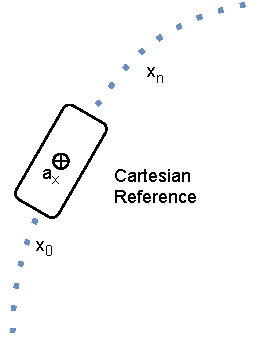
\includegraphics[width=.45\textwidth]{figs/Cartesian.drawio.pdf}
          \caption{Cartesian representation of a path}
        \end{subfigure}%
        \begin{subfigure}{.5\textwidth}
          \centering
          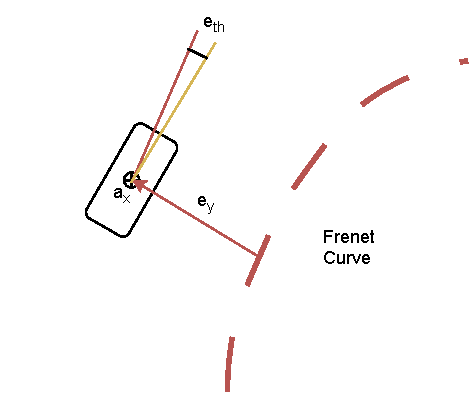
\includegraphics[width=.7\textwidth]{figs/Frenet.drawio.pdf}
          \caption{Frenet representation of a path}
        \end{subfigure}
    \caption{Two equivalent paths represented in both Cartesian and Frenet frames (Provisional) }
    \label{fig:FvC}
\end{figure}
\begin{equation}
    \label{eq:NL_model}
        \begin{aligned}
            &x = [v_x, v_y, \omega, x, y, \theta, s, e_y, \theta_e]\\ 
            &u = [\delta, a]
        \end{aligned}
\end{equation}
% \begin{equation}
%     \label{eq:NL_model}
%         x =
%         \left[\begin{array}{c}
%             v_x \\
%             v_y  \\
%             \omega  \\
%             x \\
%             y \\ 
%             \theta \\
%             s \\ 
%             e_{y}  \\
%             \theta_e 
%         \end{array}\right] , \
%         u =
%         \left[\begin{array}{c}
%             \delta \\
%             a \\
%         \end{array}\right] , \          
% \end{equation}
For clarity purposes, the continuous time non-linear model will be presented as two sets of equations. Firstly Eq. \eqref{eq:cartesian_dynamic_model} representing the Cartesian coordinates and secondly Eq. \eqref{eq:frenet_model} representing the Frenet frame coordinate set. 

\begin{subequations}
\label{eq:cartesian_dynamic_model}
\begin{equation}
    \begin{aligned}
       	& \dot v_x = a + \frac{- F_{yf} \sin{\delta} - \mu g}{m} + \omega v_y  \\
        & \dot v_y =  \frac{ F_{yf} \cos{\delta} + F_{yr}}{m} - \omega v_x \\
		& \dot \omega = \frac{ F_{yf} l_f \cos{\delta} - F_{yr} l_r}{I} \\
    	& \dot x = v_x \cos{\theta} - v_y \sin{\theta} \\
		& \dot y = v_x \sin{\theta} + v_y \cos{\theta} \\
        & \dot \theta = \omega \\
    	& \alpha_f = \delta - \tan^{-1} \left(  \frac{v_y}{v_x} - \frac{l_f \omega}{v_x} \right) \\
    	& \alpha_r = - \tan^{-1}  \left(  \frac{v_y}{v_x} + \frac{l_r \omega}{v_x} \right) \ , \
    \end{aligned}
\end{equation}
\noindent where
\begin{equation}   
	\label{eq:Pacejka_and_friction}
    \begin{aligned} 		
		&  F_{yf} = C_f \alpha_f \\
		&  F_{yr} = C_r \alpha_r \\      
    \end{aligned}
\end{equation}
\end{subequations}    

\noindent Cartesian state variables $v_x$, $v_y$ and $\omega$ represent the body frame velocities, i.e. linear in $x$, linear in $y$ and angular velocities, respectively. Accordingly, the position is defined by $x$, $y$, $\theta$ coordinates with respect to a global reference frame.
The control variables $\delta$ and $a$ are the steering angle at the front wheels and the longitudinal acceleration vector on the rear wheels, respectively.
$F_{yf}$ and $F_{yr}$ are the lateral forces produced in front and rear tires, respectively.
Front and rear slip angles are represented as $\alpha_f$ and $\alpha_r$, respectively, and $C_f$ and $C_r$ are the front and rear tire stiffness coefficients.
$m$ and $I$ represent the vehicle mass and inertia and $l_f$ and $l_r$ are the distances from the vehicle center of mass to the front and rear wheel axes, respectively. 

\begin{equation}
    \label{eq:frenet_model}
    \begin{aligned}
        & \dot s = \frac{v_x cos\theta_{e} - v_y sin\theta_{e}}{1 - e_{y} k } \\
		& \dot e_{y} = v_x \sin{\theta_{e}} + v_y \cos{\theta_{e}} \\
        & \dot \theta_{e} = \omega - \frac{v_x \cos{\theta_{e}} - v_y \sin{\theta_{e}} }{1 - e_{y} \kappa} \kappa \\
    \end{aligned}
\end{equation}
\noindent Frenet state variables are denoted as $s$, $e_{y}$ and $\theta_{e}$ and represent the position of the vehicle along the curve, the lateral error and the orientation error, respectively. Finally this model is particularised for a small scale vehicle by substituting the constants present in Table \ref{table:vehicle_parameters}. 

\begin{table}
    \caption{Dynamic model parameters of the vehicle}
    \label{table:vehicle_parameters}
    \centering
    \begin{tabular}{ l|l||l|l }
    \hline
    Parameter & Value & Parameter & Value \\
    \hline
    \hline
    $l_f$       & 0.125  $m$    & $l_r$    & 0.125  $m$  \\
    $m$         & 1.98  $kg$   & $I$      & 0.06 $kg$ $m^2$  \\
    $C_f$       & 60            & $C_r$    & 60 \\
    $\mu$ 	    & 0.05          & $g$      & 9.81 $\frac{m}{s^2}$ \\      
    \hline
    \end{tabular}
\end{table}    

\subsubsection{LPV representation}    
\label{sec:LPV}

As presented in Section \ref{sec:LPV_Mod}, we aim to reformulate the model defined by Eqs. \eqref{eq:cartesian_dynamic_model} \eqref{eq:frenet_model}
 in a pseudo-linear manner, having the rearranged model the structure of Eq.\eqref{eq:LPV_model} by using an LPV formulation. As mentioned before, this procedure is motivated by allowing the use $QP$ solvers without having a major loss in performance. 
\begin{equation}
    \label{eq:LPV_model}
    \dot x = A(\zeta) x + B(\zeta) u                 
\end{equation}
This can be done by embedding the non-linearities within varying linear parameters. Each one of these parameters is function of the vector of scheduling variables defined in Eq. \eqref{eq:scheduling_vector}, while both $ A(\zeta)$ and $B(\zeta)$ are defined in Eqs. \eqref{eq:final_LPV_A_elements} \eqref{eq:final_LPV_B_elements}, respectively. 
\begin{equation}
\label{eq:scheduling_vector}
    \zeta := \left[\begin{array}{cccccc} v_x & v_y & \theta_e & \kappa & e_y & \delta \end{array}\right]^T .
\end{equation}

\noindent\begin{minipage}{.5\linewidth}    
    \begin{equation}
        \label{eq:final_LPV_A_elements}
        A(\zeta) =	\left[\begin{array}{ccccccccc}
                    A_{11}  & A_{12}    & A_{13}    & 0 & 0  & 0 & 0 & 0 & 0 \\
                    0       & A_{22}    & A_{23}    & 0 & 0  & 0 & 0 & 0 & 0 \\
                    0       & A_{32}    & A_{33}    & 0 & 0  & 0 & 0 & 0 & 0  \\
                    A_{41}  &  A_{42}    & 0    &  0  &  0  & 0 & 0  & 0 & 0   \\
                    A_{51}   & A_{52}    & 0  & 0 & 0 & 0 & 0  & 0 & 0\\
                    0  & 0    & 1 & 0 & 0  & 0 & 0  & 0 & 0 \\ 
                    A_{71}       & A_{72}    & 0    & 0 & 0 & 0 & 0 & 0 & 0    \\
                    A_{81}  & A_{82}    & 0 & 0 & 0  & 0 & 0  & 0 & 0  \\ 
                    A_{91}        & A_{92}    & 1    & 0 & 0 & 0 & 0 & 0 & 0   \\
        \end{array}\right]
   \end{equation}
\end{minipage}%
\begin{minipage}{.5\linewidth}  
   \begin{equation}
        \label{eq:final_LPV_B_elements}
        B(\zeta) = \left[\begin{array}{cc}
                    -\frac{1}{m} \sin{\delta} C_f & 1 \\
                    \frac{1}{m} \cos{\delta} C_f & 0 \\
                    \frac{1}{I} \cos{\delta} C_f l_f  & 0 \\
                    0 & 0 \\
                    0 & 0 \\
                    0 & 0 \\
                    0 & 0 \\
                    0 & 0 \\
                    0 & 0 
        \end{array}\right] 
    \end{equation}
\end{minipage}\\

\noindent where $A_{ij}$ are defined as

\begin{equation*}	
    \begin{array}{ccc}		
    
        A_{11} =  -\mu g   &, A_{12} = \frac{C_f \sin{\delta} }{m v_x} &, A_{13} = \frac{C_f l_f \sin{\delta} }{m v_x} + v_y \\
        A_{22} =  -\frac{ C_r + C_f \cos{\delta} }{m v_x} &, A_{23} = -\frac{ C_f l_f \cos{\delta} - C_r l_r }{ m v_x } - v_x \\ 
        A_{32} = -\frac{ C_f l_f \cos{\delta} - l_r C_r }{ I v_x } &, A_{33} = -\frac{ C_f l_f^2 \cos{\delta} + l_r^2 C_r }{ I v_x } \\
        A_{41} =  cos(\theta) &, A_{42} = -sin(\theta)\\
        A_{51} = sin(\theta) &, A_{52} = cos(\theta)\\
        A_{71} =  \frac{cos(\theta_e)}{1-e_{y}_k} &, A_{72} =  -\frac{sin(\theta_e)}{1-e_{y}_k}\\
        A_{81} =  -sin(\theta_e) &, A_{82} = cos(\theta_e)\\
        A_{91} = -\frac{ \kappa }{(1 - e_{y} \kappa) }\cos{\theta_{e} &, A_{92} = \frac{ \kappa }{(1 - e_{y} \kappa) } \sin{\theta_{e}}
    
    \end{array}
\end{equation*}

As a final remark, it can be seen that the proposed model depends on $\zeta$, which can not be updated while solving the optimisation problem in a linear manner. Thus an approximated version of $\hat{\zeta}$ is used, which we can compute by no considering the current values of the scheduling variables but its prediction computed in previous iterations. This assumption is widely accepted within the control community, being some examples already cited in previous sections of this paper. Moreover, in \cite{alcala2020autonomous} this same approach was used successfully in autonomous racing, a more challenging driving situation, which suggests the viability of this assumption considering reasonable times between consecutive executions of the algorithm. All the variables presented in this section are graphically displayed in the system model of Figure \ref{fig:model}. 

\subsubsection{Environment modelling}    

The reference to be followed by our fleet of agents is modelled through a set of curves of constant curvature $k$ and a given length $l$. This is embedded into the model by the time-varying constant $k$ and the state variables $s$, $e_{y}$ and $\theta_{e}$. In order to update the parameter $k$ a greedy search is performed through the set of curves seeking the one that encloses the current position of the vehicle, taking into account the Frenet frame state variables. By considering the previous position and taking into account that each segment has a constant curvature we can perform this search locally without having a major impact on the algorithm computational time. Note that the correctness of $k$ is subject to the precision of the state variable $s$ which in a real scenario will depend on both the model quality and the precision of the onboard localisation module.\\

In this particular work we assume that the reference curves are computed offline, resembling what could be a segment of a highway, as presented in Fig. \ref{fig:Highway}. This same approach has been extensively used in the past, either by assuming prior knowledge of the track \cite{alcala2020lpv} or through an online estimation \cite{Kabzan2019}. However, it is not trivial to expand it to the autonomous driving domain, as shown in \cite{li2020fast} the resulting Frenet curves may degrade in the presence of large road curvatures. Thus, we assumed a suitable set of reference curves and left as future work the interface of our local planning algorithms with a global planner capable of handling the degradation of Frenet frame reference. It is worth to note that this is an active research line, being of special interest the algorithm proposed by \cite{Sun2020}, which allows to convert an arbitrary Cartesian reference into an usable curve while preventing this degradation. 

\begin{figure}
    \centering
        \begin{subfigure}{0.5\textwidth}
          \centering
          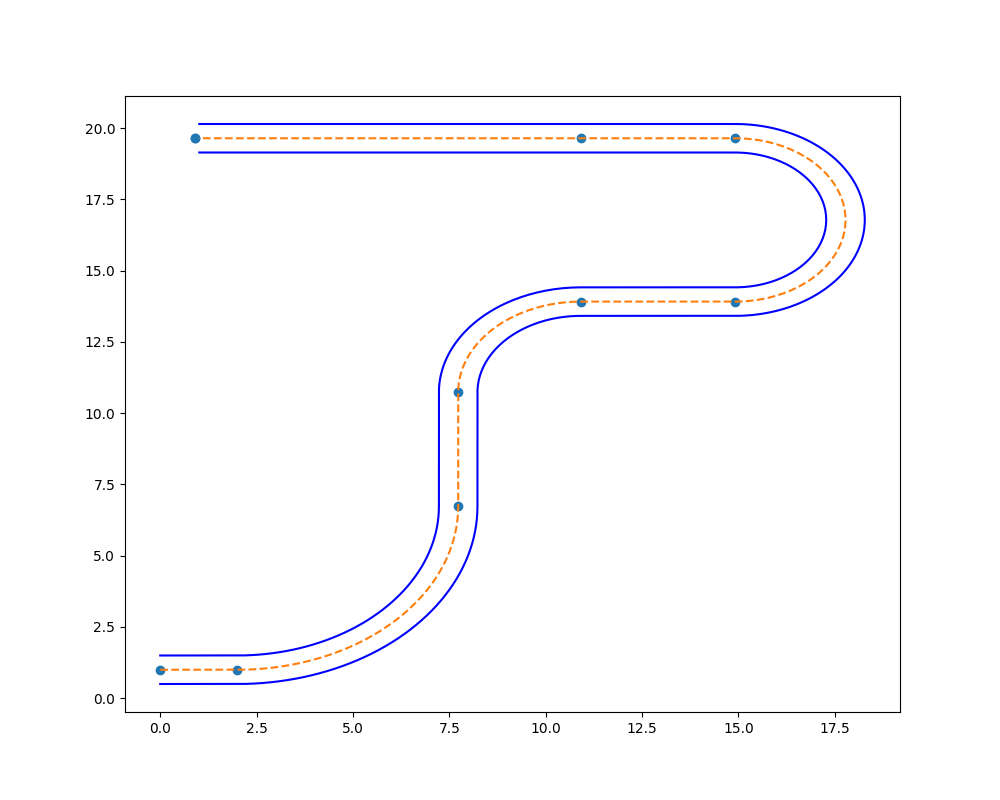
\includegraphics[width=\textwidth]{figs/map.png}
          \caption{Highway map}
          \label{fig:Highway}
        \end{subfigure}%
        \begin{subfigure}{.5\textwidth}
          \centering
          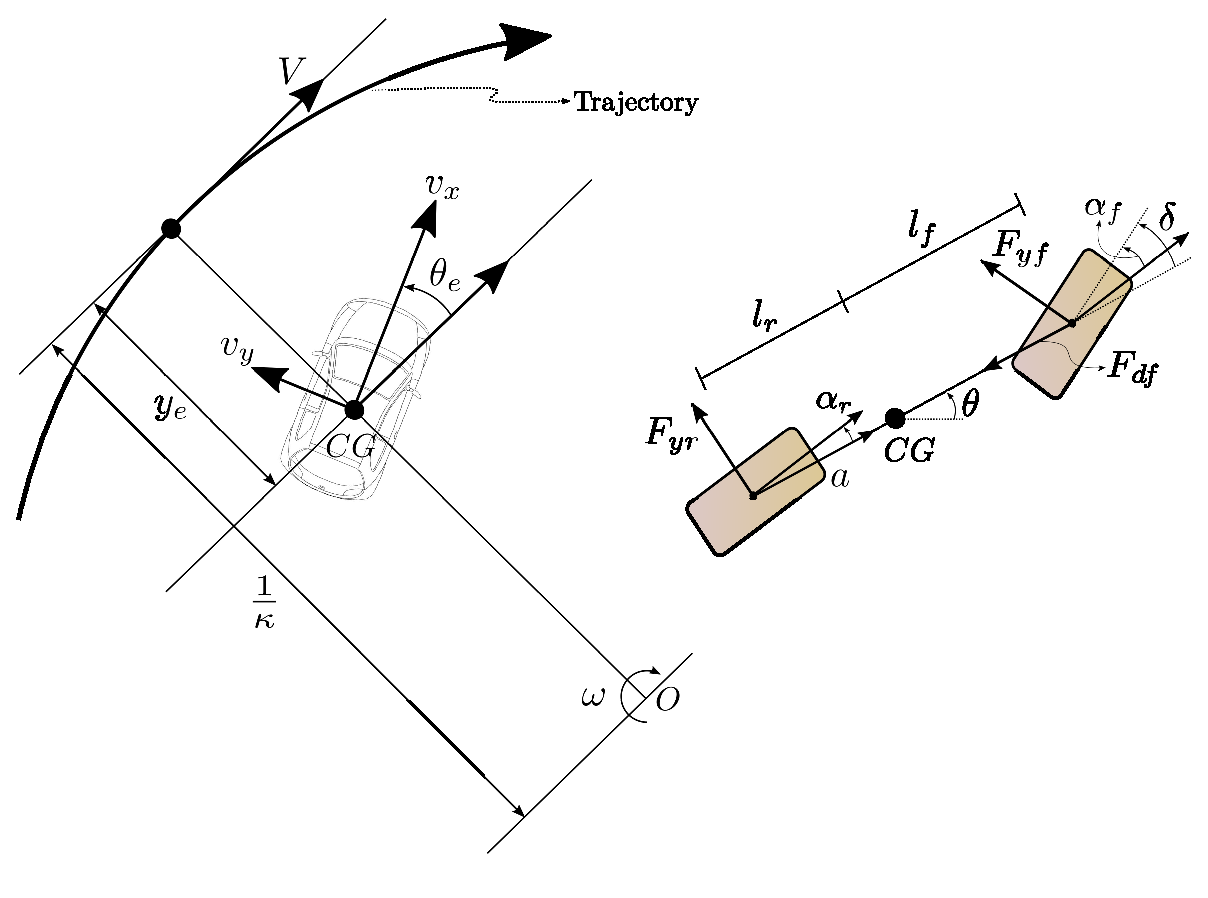
\includegraphics[width=\textwidth]{figs/variables_representation.eps}
          \caption{Agent variables representation from \cite{racingEM}}
          \label{fig:model}
        \end{subfigure}
    \caption{Case study scenario representing a Highway }
    \label{fig:FvC}
\end{figure}

% ------------------------------------------------------------------------------
% ------------------------------------------------------------------------------


\section{Experiments and results}
\label{seq:exp}
The effectiveness of both algorithms presented in Section \ref{Sec:MA optimal plans} is going to be assessed by applying them in the scenario presented in Section \ref{sec:modeling}. We aim to test their viability and asses whether or not there is a performance loss after applying the relaxation proposed in Section \ref{sec:LPV - DMPC}. Furthermore, other metrics such as the computational time, vehicle states and other valuable insights are going to be presented. It is worth to mention that we ruled out the optimal hyperplane approach presented in Section \ref{NL MPC}, as the computational times involved in the optimisation proved to be prohibitive compared to its Euclidean formulation without any remarkable performance improvements. Thus, we decided to continue the comparison using only the later algorithm and its pseudo-linear counterpart.\\

The results presented in this section where generated using OSQP and CASADI, as quadratic and non-linear solvers respectively. The code was deployed in a ROS network where each agent acts as an individual computing thread, resembling a real network of autonomous agents. All the computing times presented in this section do not include communication delays, as they are negligible in the simulation platform, however they should be taken into consideration for any practical implementation. Finally, all tests were carried out in a consumer laptop with 16Gb of RAM, an i7-13700H CPU and no specific hardware acceleration.\\ 

The main differences between an LPV-DMPC and a NL-DMPC are whether or not we trade-off some performance for computational time. In particular, the relaxation applied to the LPV-DMPC to make the obstacle avoidance quadratic implies that we are decoupling the system and no longer have an implicit collaboration between agents, we only consider their trajectories as limitations in the free space. On the other hand, by applying the strict NL-DMPC we find the trajectories that globally minimise a cost function involving all the individual agents, however this implies solving several iterations of a distributed optimisation problem, which naturally imply $N$ communication delays and using a solver that is slower than its quadratic counterpart due to the inherently complexity of non-linear problems. In fact, solving the non-linear formulation is a NP-Hard problem \cite{nl_time} while the proposed quadratic problem can be solved in weakly polynomial time \cite{poly_time} due to the convexity of its cost function. The metrics used for the sake of the comparison are the 2D generated path, the safety limits, the look-ahead distance and the computational time per iteration. As we can see in Figure \ref{fig:GeneratedPlans} both algorithms lead to similar paths from a general point of view and we can not state any performance difference as both would successfully solve the problem. However it is worth to note that agents using the LPV-DMPC end the experiment slightly faster, in the specific experiment used in this Section this difference was of $6.57s$ under similar tuning conditions.\\ 

\begin{figure}
    \centering
        \begin{subfigure}{0.5\textwidth}
          \centering
          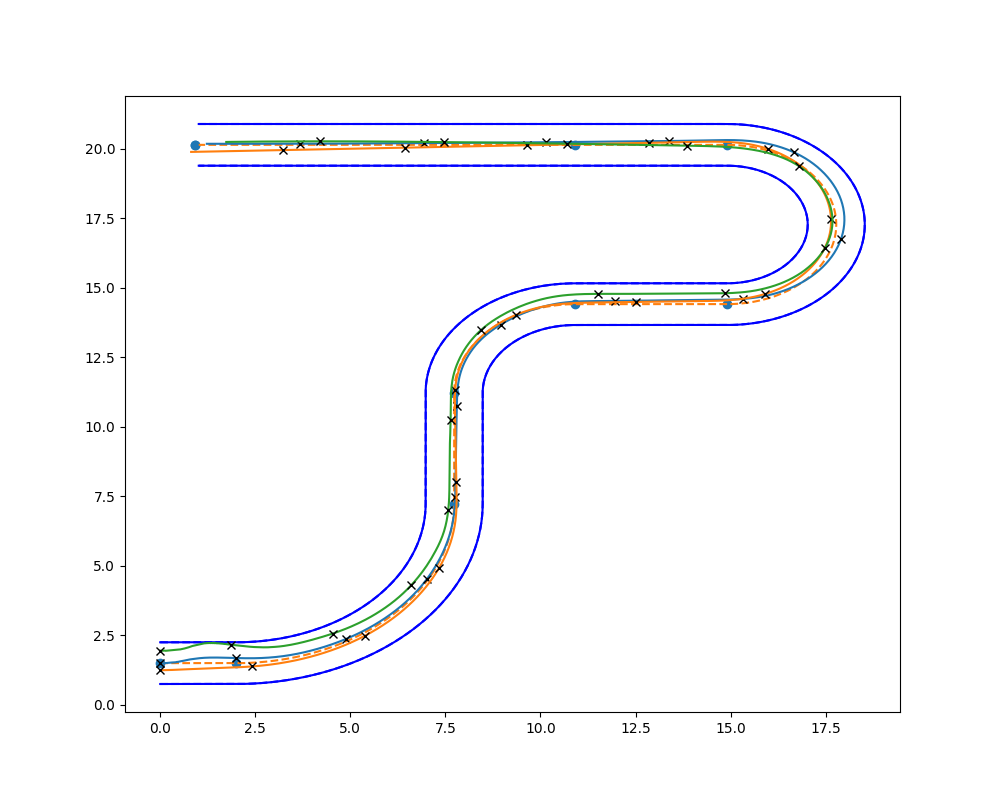
\includegraphics[width=\textwidth]{figs/experiments/track_LPV.png}
          \caption{LPV-DMPC}
          \label{fig:figPlane}
        \end{subfigure}%
        \begin{subfigure}{.5\textwidth}
          \centering
          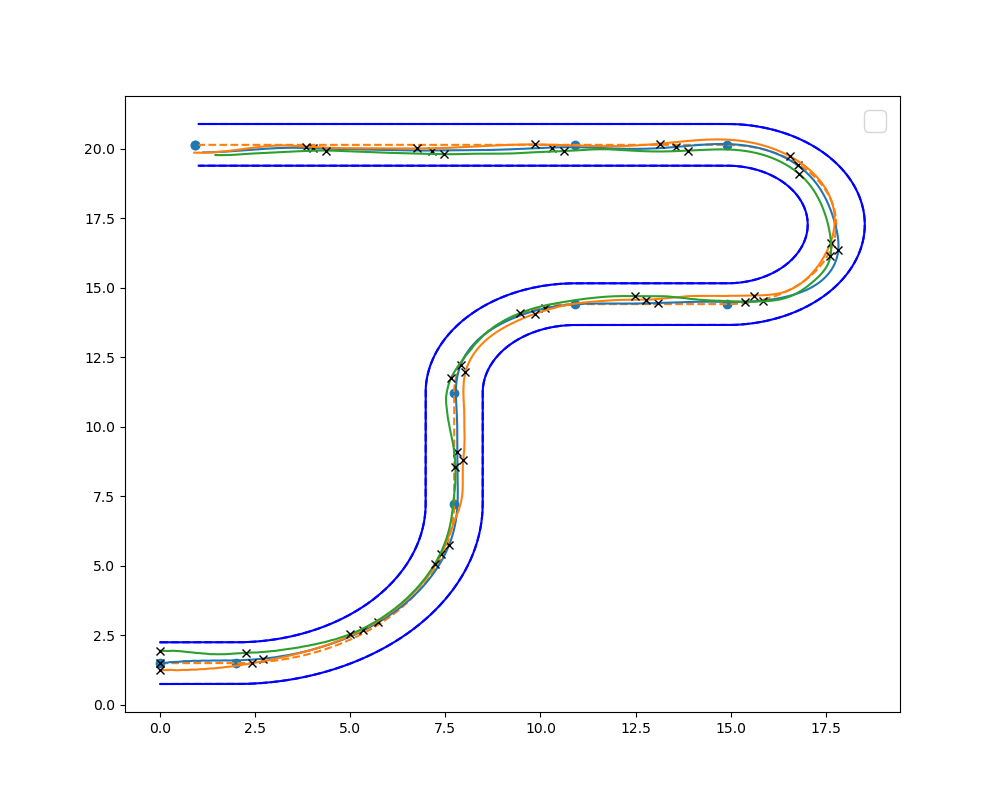
\includegraphics[width=\textwidth]{figs/experiments/track_NL.png}
          \caption{NL-DMPC}
          \label{fig:figEuclidean}
        \end{subfigure}
    \caption{Comparison of platoon generated plans}
    \label{fig:GeneratedPlans}
\end{figure}

% \begin{figure}[h]
%     \centering
%     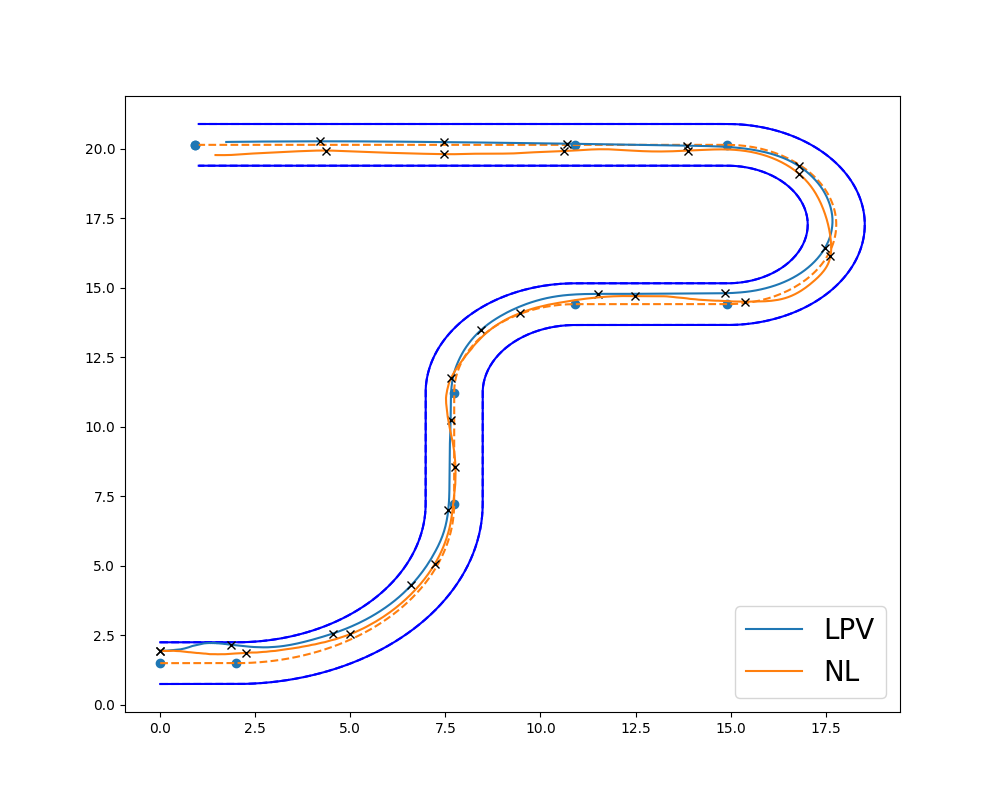
\includegraphics[width=.55\textwidth]{figs/experiments/track_ta.png}
%     \caption{Single agent trajectory, NL-DMPC vs LPV-DMPC }
%     \label{fig:SAexp}
% \end{figure}

As mentioned before, in order to asses performance differences we will use $v_x$ and both inter-vehicular and look-ahead distances. This selection is motivated by the fact that we aim to know how fast are we going to reach our goal and how safe is the trajectory going to be. It is trivial to see that higher linear velocities will lead to shorter trajectories. The selection of the safety metrics aim to represent how well can we react to unforeseen scenarios. Specifically, how far away can a detectable obstacle be to be considered in the plans and what margin do we have in the face of events such as an agent losing control of the vehicle or an animal crossing the road. Firstly, as we can see in Figure \ref{fig:Vcomp} in both cases agents keep a velocity around the road limits, which in this case is set to $3 m/s$, however that is not a hard constraint and higher velocities are accepted. Again we can not conclude any major benefit of using either of the approaches, however it is worth to note that as we enforce a specific formation in the decentralised formulation their velocities tend to vary less that in the distributed counterpart, either behaviour can be enforced by the fine tunning of cost functions.\\ 

\begin{figure}[h]
    \centering
    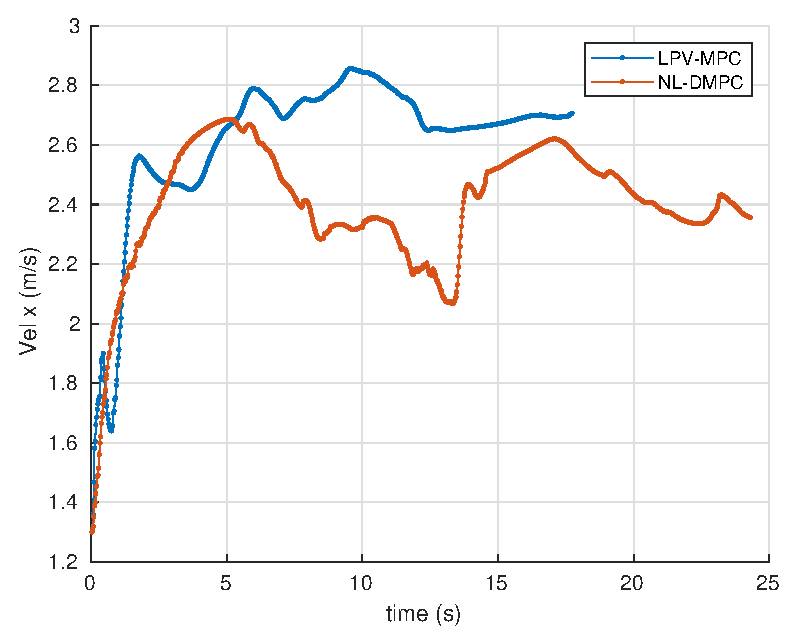
\includegraphics[width=.43\textwidth]{figs/experiments/vel.eps}
    \caption{Velocity profile comparison between algorithms }
    \label{fig:Vcomp}
\end{figure}

Secondly, as we can see in Figure \ref{fig:Dcomp} the LPV-MPC converges into a formation, which is encouraged by the cost function. On the other hand, in the NL-DMPC agents reconfigure on the fly, leading to a less stable inter-vehicle distance disposition. Again, either behaviour can be enforced through modifying the cost function accordingly, so it is given as a decision of the designer which is more desirable in their application. However, we can see how in both cases the algorithms successfully respect the security margins. In terms of the look-ahead distance we can see how the LPV-DMPC predicts further in the future due to the longer prediction horizon, as in the LPV case we use up to 120 steps and in the NL counterpart 20. It is worth to note than in strict theory we should be able to match both prediction horizons, however this would make solving the non-linear case prohibitively costly and may lead to a degraded solution. For instance, we have encountered cases where even with a high number of solver iterations, around 100k, the solution is not accurate enough and compromises the algorithm, being the only workaround to use smaller horizons to reduce the complexity of problem. It is trivial to see how the simplicity of the LPV counterpart provides an advantage by allowing to increase the horizon, thus computing more refined plans. \\ 

\begin{figure}[h]
    \centering
        \begin{subfigure}[a]{0.5\textwidth}
          \centering
          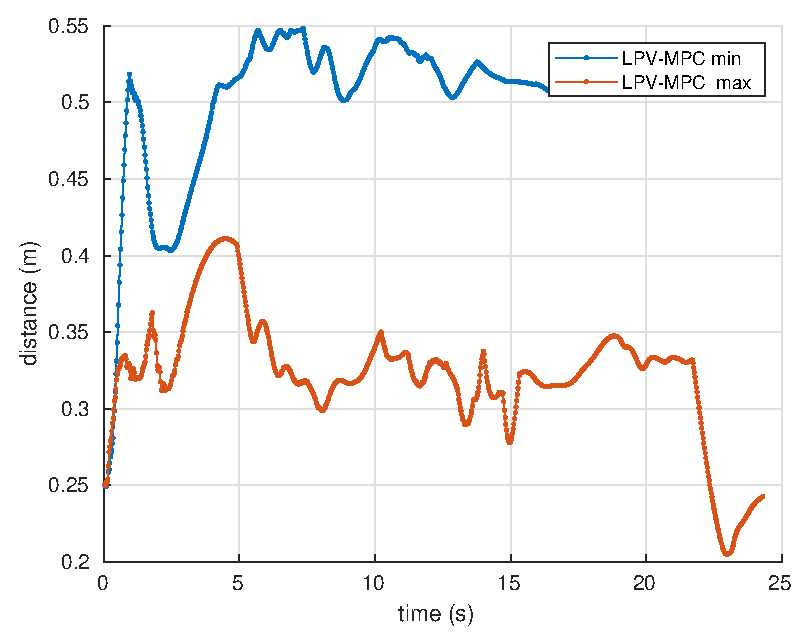
\includegraphics[width=0.9\textwidth]{figs/experiments/d_min.eps}
          \caption{Minimum inter-vehicular distance}
          \label{fig:figPlane}
        \end{subfigure}%
        \begin{subfigure}[a]{.5\textwidth}
          \centering
          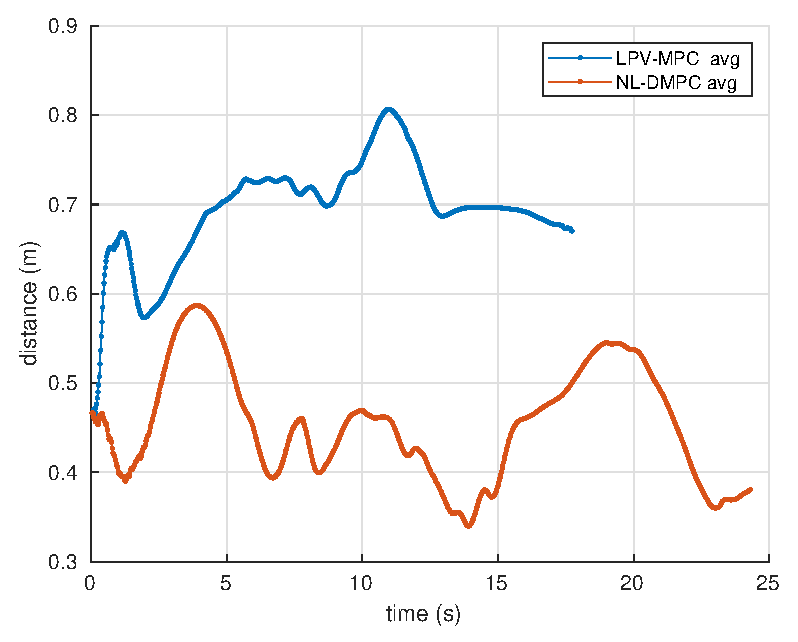
\includegraphics[width=0.9\textwidth]{figs/experiments/d_avg.eps}
          \caption{Average inter-vehicular distance}
          \label{fig:figEuclidean}
        \end{subfigure}
        \begin{subfigure}[b]{0.5\textwidth}
          \centering
          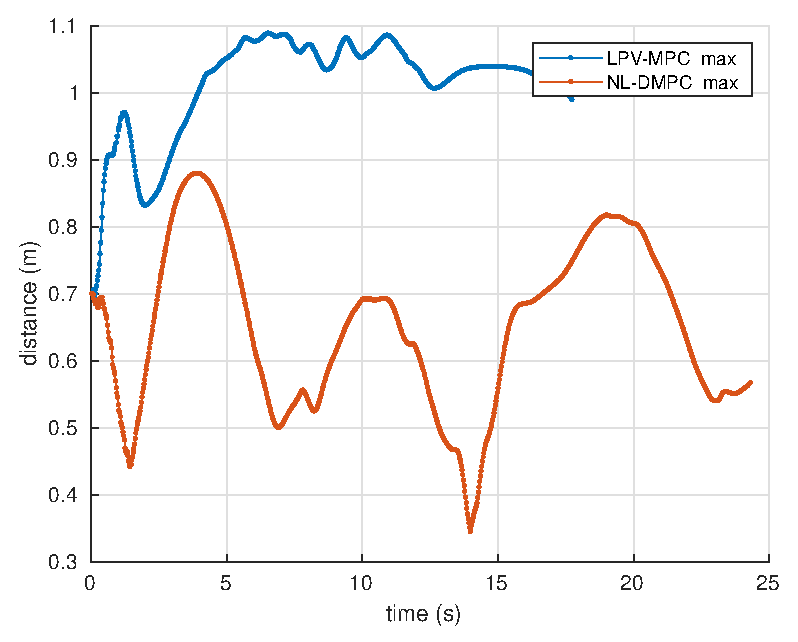
\includegraphics[width=0.9\textwidth]{figs/experiments/d_ma.eps}
          \caption{Maximum inter-vehicular distance}
          \label{fig:figPlane}
        \end{subfigure}%
        \begin{subfigure}[b]{.5\textwidth}
          \centering
          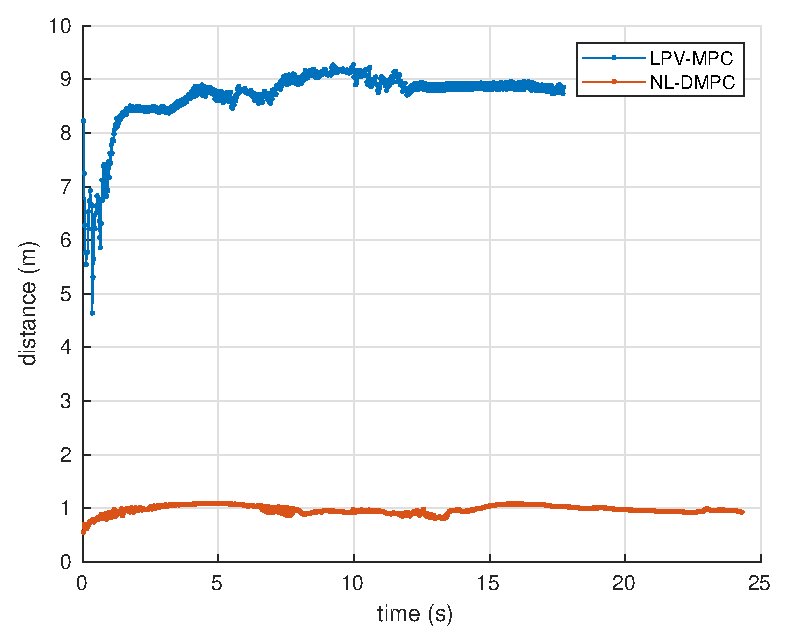
\includegraphics[width=0.9\textwidth]{figs/experiments/la_avg.eps}
          \caption{Look-ahead distance}
          \label{fig:figEuclidean}
        \end{subfigure}
    \caption{Comparison of distance metrics}
    \label{fig:Dcomp}
\end{figure}

Finally, as we mentioned before the LPV formulation vastly improves the computational times of its non-linear counterpart, as it can be seen in Figure \ref{fig:Tcomp}, in this particular case the LPV implementation is four times faster than its distributed counterpart. Note that Figure \ref{fig:Tcomp_ZIN} represents the computational burden after a warm up stage, where a formation is acquired by the agents. As an additional remark, the computational time of the OCD algorithm is sensible to the convergence rate in the particular scenario, for instance and after fine-tuning we achieved convergence in four iterations, thus limiting the computational time of the problem. On the other hand, with the LPV counterpart the computational time will always be bounded by the time required to find a feasible solution to Eqs. \eqref{eq:plane_computation} \eqref{eq:LPV_MPC}. Note that in both cases there is an struggle in solve the initial iterations, as agents are gathered together close to the collision distance, but it is specially relevant in the case of the quadratic solver, being the first iterations ten times slower.\\ 

\begin{figure}[h]
    \centering
        \begin{subfigure}{0.5\textwidth}
        \centering
        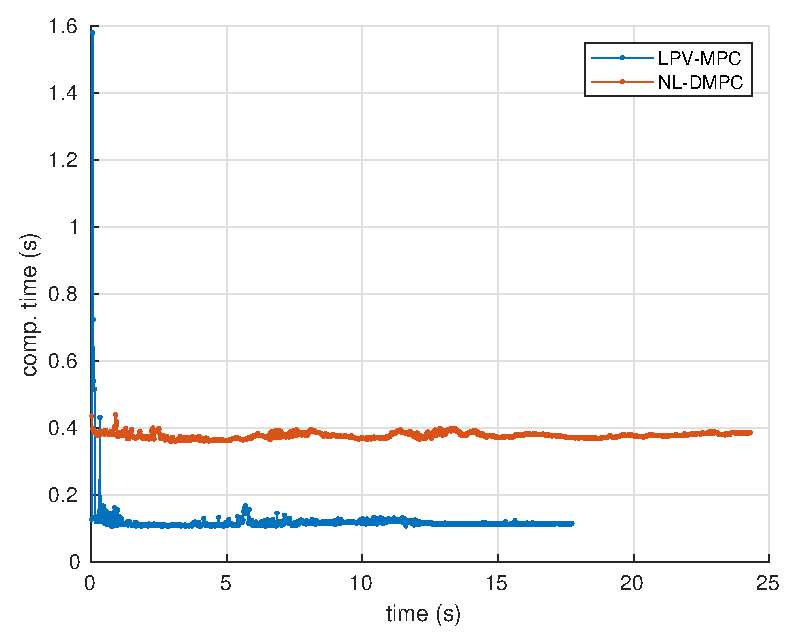
\includegraphics[width=.9\textwidth]{figs/experiments/t_avg.eps}
        \caption{Computational time of the algorithms }
        \label{fig:Tcomp}
        \end{subfigure}%
        \begin{subfigure}{.5\textwidth}
        \centering
        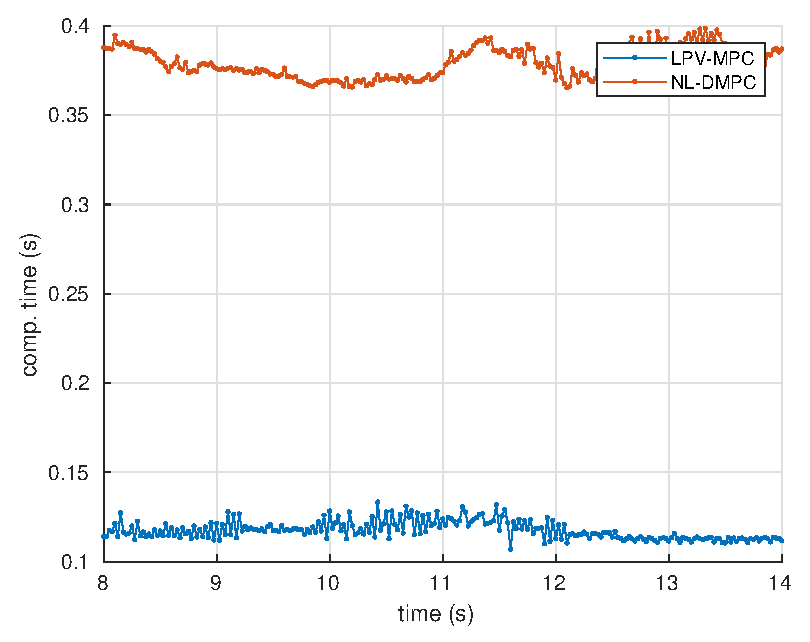
\includegraphics[width=.9\textwidth]{figs/experiments/t_avg_zn.eps}
        \caption{Computational time of the algorithms in formation}
        \label{fig:Tcomp_ZIN}
        \end{subfigure}
    \caption{Computational time comparison}
    \label{fig:Dcomp}
\end{figure}

As final remarks, we can say that the LPV approach is generally more appealing due to its computational robustness and simplicity. However, from a strict point of view it is closer to an accurate obstacle avoidance than to a distributed optimisation problem per se. On the other hand, we saw how solving a distributed problem implies a higher computational cost that poorly scales with the number of agents, but allows solving it from a global point of view. Furthermore, even if in this case the benefits of the distributed counterpart could not observed we can not rule them out, as other metrics such as fuel consumption happened to improve in other works. 
%------------------------------------------------------------------------------
\section{Conclusions and future work}
\label{sec:Conclusions} 

In this paper we developed a non-linear distributed MPC and proposed a relaxed version which allows solving the problem in a quadratic fashion. Furthermore, both algorithms were implemented and tested in a distributed manner in a ROS network, mimicking the physical layout of a platoon of autonomous vehicles. After testing them in a scenario resembling a highway in Section \ref{seq:exp} we saw that both approaches present a similar behaviour, agents reach some sort of formation and stay in it while traversing the environment while satisfying the safety conditions.\\ 

In general, we can say that the simplicity and robustness of solving a quadratic problem is preferable to its non-linear counterpart in the autonomous driving problem. Furthermore, we did not measure any remarkable performance improve between them. However, as mentioned before, relaxing the distributed optimisation into isolated problems conflicts the collaborative nature of the project, as they do not interact in a peer-to-peer basis but in an individualistic approach. After this research we concluded that even-though the collaborative local planning has interesting properties, after fine-tuning of the OCD algorithm we did not manage to provide a equivalent alternative to its decentralised counterpart in terms of computational time. All in all, the LPV formulation is more reliable due to its optimisation design and requires less communication, while the NL-DMPC is more fragile as is dealing with an NP-Hard problem that may require a large number of iterations, and their subsequent communications delays, to converge into an optimal solution. However, the latter presents a global collaboration not present in the former. Among all the possible scenarios we studied the simplest one, which does not strictly involve any interaction other than inter-vehicle obstacle avoidance, leaving room for improvements and situations that may not be solvable by the LPV-DMPC as it is.\\ 

Collaboration is still a key, if not mandatory, element in most autonomous driving situations where agents have individual goals and the environment forces individual agents to interact so that deadlocks and collisions are prevented. In those cases, inter-agent coupling can not be relaxed in the way we did in LPV-MPC; agents need to actively collaborate to overcome this situations. For that reason, we aim to expand the algorithms presented in this paper by exploring other applications of OCD. We have seen how over-complicating the formulation leads to intractable, if not unsolvable, optimisation problems that have little to no application outside of simulated environments. As a consequence, we aim to expand this research by apply variations of both LPV-DMPC and NL-DMPC in a cascade fashion so that the collaborative decisions can be taken in a higher level, less constraining in terms of computational time, while the local safety is ensured by a faster distributed planner.

\bibliographystyle{cas-model2-names}
\bibliography{cas-refs}

% ------------------------------------------------------------------------------
% ------------------------------------------------------------------------------


\end{document}
